\section{Evaluation}
We cannot rely on traditional approaches such as manual
labeling to evaluate large-scale performance.  We therefore sought to
minimize failure rate, quantify the repeatability of cortical
thickness measures, test accuracy in BrainAGE \citep{franke2010} and
determine whether the DiReCT pipeline reveals biologically plausible relationships
between the cortex, age and gender.  Collectively, these surrogate
measurements allow us to establish data-derived performance standards.

\subsection{Computation Time and Failure Rate}
All images underwent the pipeline processing illustrated in Figure 
\ref{fig:pipeline} using the computational cluster at the University 
of Virginia.%
\footnote{
http://www.uvacse.virginia.edu/itc-clusters/
}  
Processing times varied approximately between 10--20 hours per subject
for the entire cortical thickness estimation procedure.  The propagation of the
NIREP labels to each subject using label fusion as described earlier
was performed in parallel and took anywhere between 40 and 80 hours per 
subject for 16 serial image registrations and the joint label fusion \citep{wang2013}.%
\footnote{
All processing on the UVA cluster was set to be single-threaded with a maximum requested memory footprint of 8 GB.  See script for exact cluster commands.
}  
Average thickness values were tabulated per subject for each of the
32 NIREP labels.  Cerebral volumes for each subject derived from the brain 
extraction step were also calculated.  All these data were written to separate csv
files corresponding to data set for subsequent 
analysis (also included with the scripts).  Visual sample results from each data set are provided in 
Figure \ref{fig:sampleResults}.

\begin{figure}
  \begin{center}
  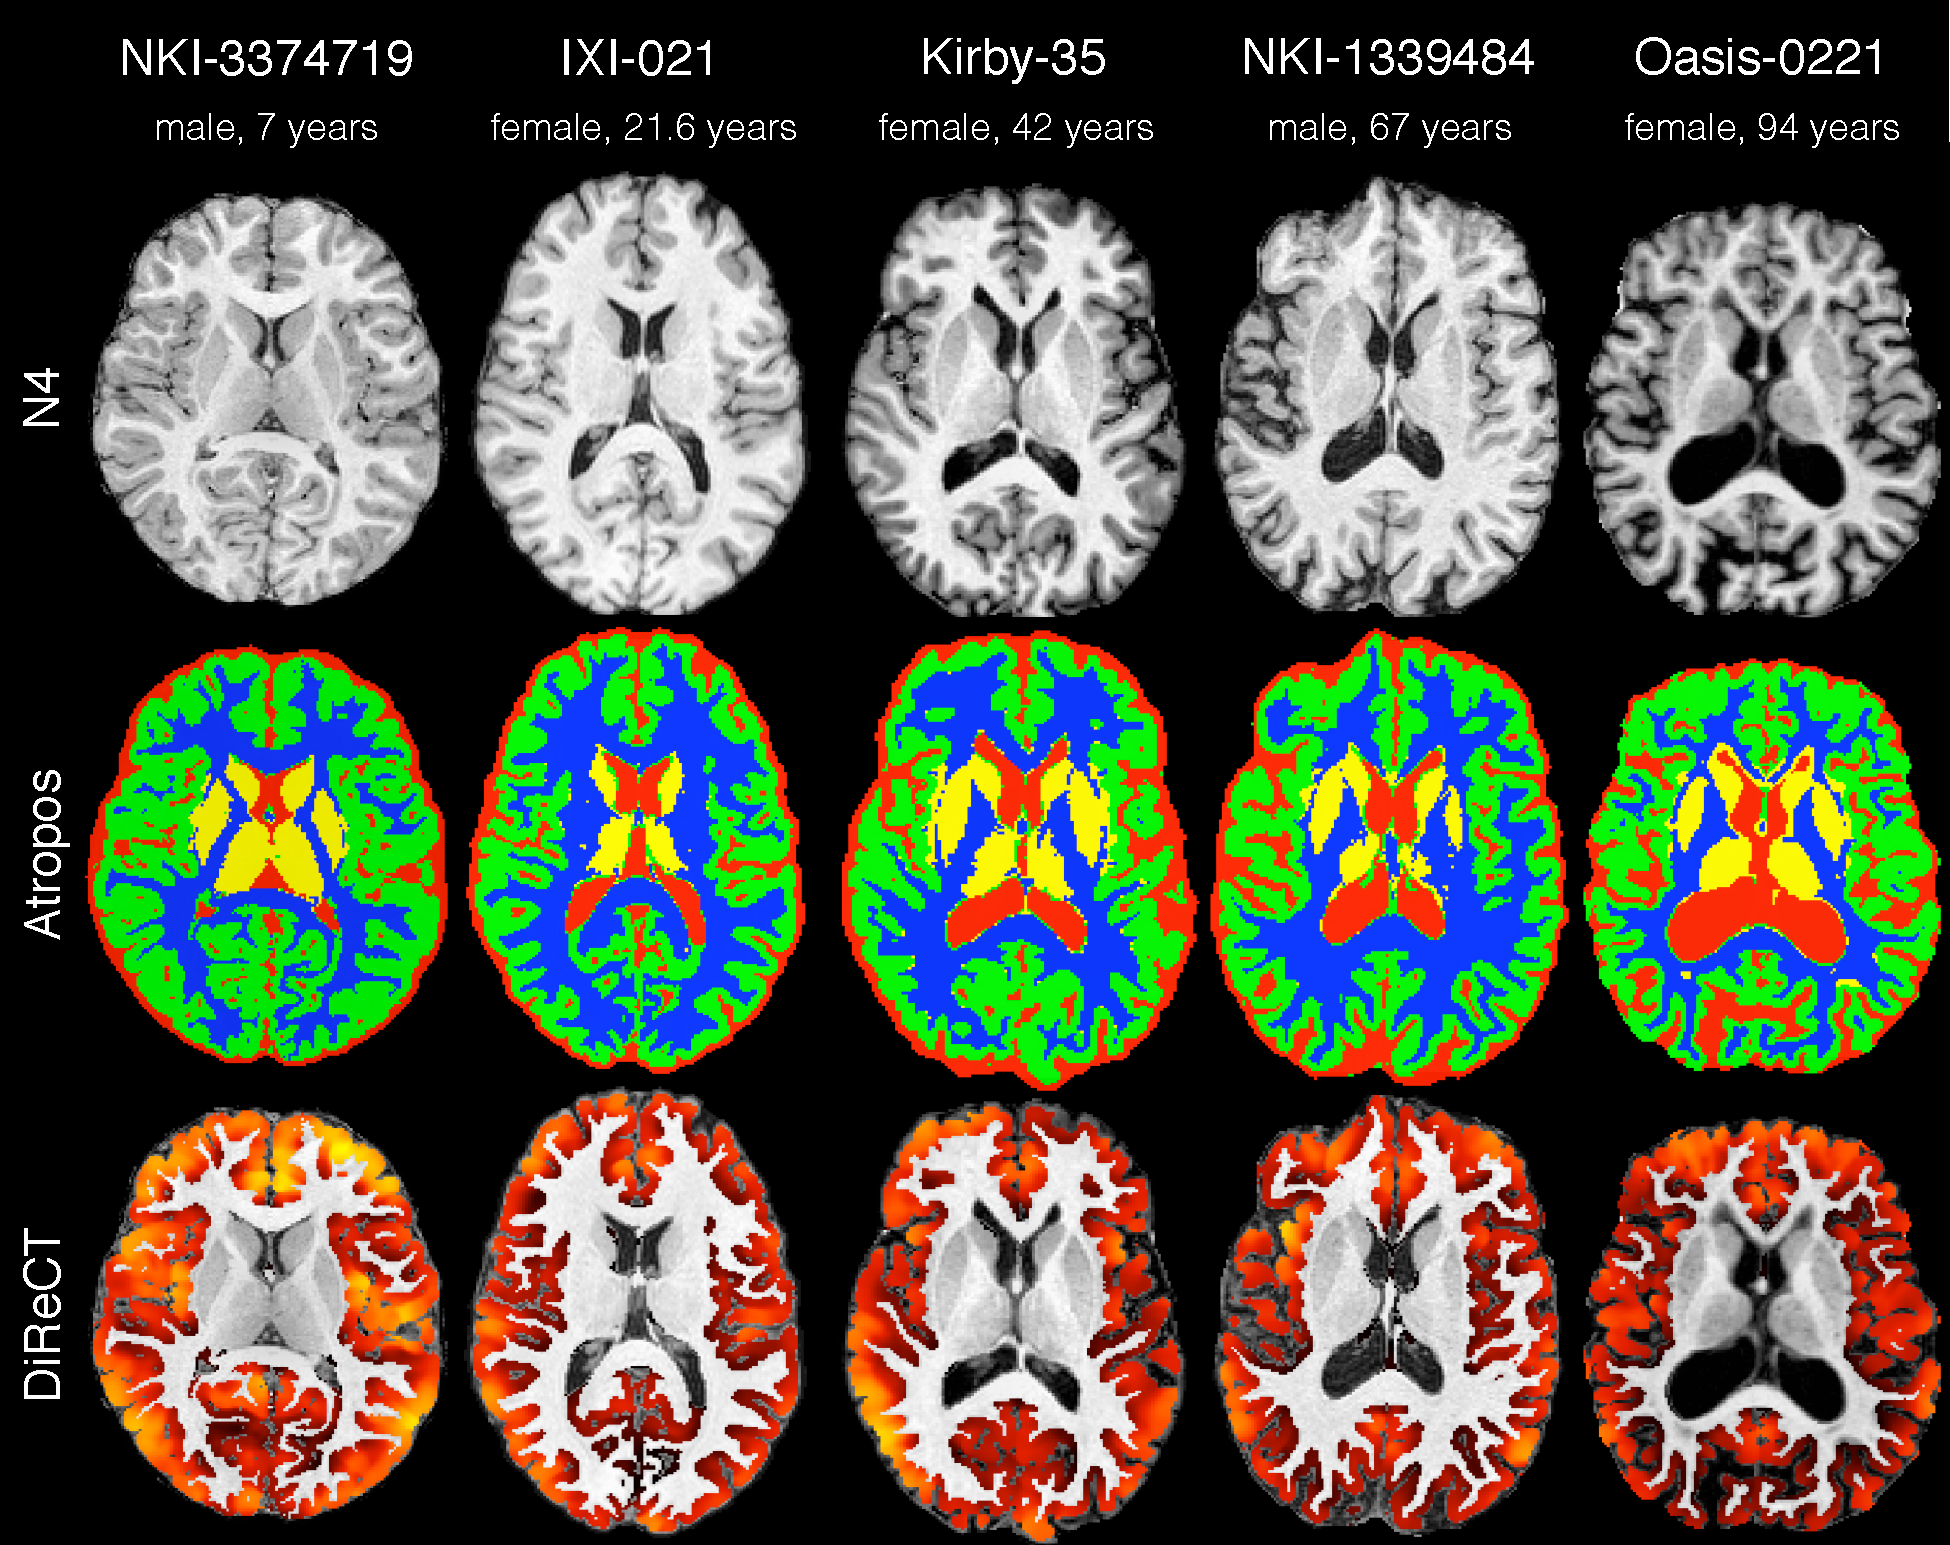
\includegraphics[width=130mm]{sampleVisualResults.pdf}
  \caption{Sample results from each of the four data sets showing the N4 bias
  corrected images, 3-tissue segmentation, and cortical thickness maps.}
  \label{fig:sampleResults}
  \end{center}
\end{figure}

%We visually inspected the brain extraction, the estimated brain volume
%and cortical thickness measurements for each of the 1205 images.  Out
%of 1205 images, only 2 subjects failed (0.16\% failure rate).
%\textcolor{red}{ Nick - can you explain this further ?  } 
  
  
\subsection{Reproducibility}

\begin{table}
\centering
\begin{tabular*}{\textwidth}{@{\extracolsep{\fill}} l c c c c}
\toprule
\multicolumn{1}{c}{} & \multicolumn{2}{c}{Absolute Difference (mm)} & \multicolumn{2}{c}{Percent Variability Error} \\
\multicolumn{1}{c}{Region} & \multicolumn{1}{c}{Left} & \multicolumn{1}{c}{Right} & \multicolumn{1}{c}{Left} & \multicolumn{1}{c}{Right} \\
\midrule
occipital & $0.16 \pm 0.21$ & $0.17 \pm 0.22$ & $5.36 \pm 6.92$ & $5.79 \pm 7.17$\\
cingulate & $0.12 \pm 0.13$ & $0.12 \pm 0.14$ & $3.7 \pm 4.49$ & $3.62 \pm 4.6$\\
insula & $0.18 \pm 0.17$ & $0.17 \pm 0.17$ & $4.52 \pm 4.27$ & $4.43 \pm 4.36$\\
temporal pole & $0.23 \pm 0.23$ & $0.21 \pm 0.2$ & $4.93 \pm 5.48$ & $4.81 \pm 5.01$\\
superior temporal & $0.13 \pm 0.15$ & $0.1 \pm 0.13$ & $4.74 \pm 5.34$ & $3.58 \pm 4.92$\\
infero temporal & $0.26 \pm 0.32$ & $0.24 \pm 0.31$ & $6.86 \pm 8.8$ & $6.58 \pm 9.21$\\
parahippocampal & $0.2 \pm 0.19$ & $0.18 \pm 0.15$ & $5.13 \pm 5.29$ & $4.61 \pm 3.76$\\
frontal pole & $0.23 \pm 0.24$ & $0.24 \pm 0.25$ & $7.1 \pm 8.07$ & $7.4 \pm 8.32$\\
superior frontal & $0.11 \pm 0.12$ & $0.12 \pm 0.12$ & $3.86 \pm 4.48$ & $3.85 \pm 4.31$\\
middle frontal & $0.17 \pm 0.2$ & $0.16 \pm 0.21$ & $6.58 \pm 7.8$ & $5.87 \pm 7.96$\\
inferior & $0.12 \pm 0.15$ & $0.12 \pm 0.16$ & $4.53 \pm 5.53$ & $4.26 \pm 5.49$\\
orbital frontal & $0.16 \pm 0.2$ & $0.19 \pm 0.18$ & $4.77 \pm 6.12$ & $5.39 \pm 5.36$\\
precentral & $0.11 \pm 0.11$ & $0.11 \pm 0.13$ & $4.46 \pm 4.5$ & $4.15 \pm 4.81$\\
superior parietal & $0.09 \pm 0.1$ & $0.09 \pm 0.09$ & $3.71 \pm 4.14$ & $3.67 \pm 3.78$\\
inferior parietal & $0.14 \pm 0.17$ & $0.13 \pm 0.18$ & $4.96 \pm 6.06$ & $4.96 \pm 6.74$\\
postcentral & $0.13 \pm 0.16$ & $0.14 \pm 0.14$ & $5.51 \pm 6.32$ & $6.02 \pm 6.01$\\
\bottomrule
\end{tabular*}
\caption{Mean absolute difference and percent variability error ($\pm$ standard deviation) of repeated 
cortical measurements for both the Oasis and Kirby repeat scans.
These differences were not statistically significant (two-tailed $t$-test
with false discovery rate (FDR) multiple comparisons correction).
}
\label{table:error}
\end{table}

Repeat scans of 40 subjects (20 Kirby subjects and 20 Oasis subjects) were 
used to determine the reproducibility of regional cortical thickness 
measurements. Similar to the assessment given in \cite{jovicich2013}, we
show regional reproducible thickness measurements, $T$, in terms of the
variability error:
\begin{align}
\varepsilon = \frac{|T_{scan} + T_{rescan}|}{0.5 \times (T_{scan} + T_{rescan})}.
\end{align}
Error values (including absolute mean differences) for the 32 NIREP regions for both the Oasis and Kirby reproducibility data sets
are given in Table \ref{table:error}.  We also calculated the intraclass 
correlation coefficient 
(``ICC(2,1)'' in the notation of \cite{shrout1979}) to assess scan/rescan
reliability which showed reliable agreement ($ICC=0.95$).  Additional regression
testing exploring the effects of site, age, and gender demonstrated no statistically significant effect on regional mean thickness difference.

\subsection{BrainAGE Evaluation}


\begin{table}
\centering
\begin{tabular*}{0.9\textwidth}{@{\extracolsep{\fill}} l c c}
\toprule
\multicolumn{1}{c}{Analysis} & \multicolumn{1}{c}{$r$} & \multicolumn{1}{c}{mean error (years)} \\
\midrule
Gray matter probability & 0.93 & 6.17 \\  
Cortical thickness & 0.90 & 7.19 \\
\bottomrule
\end{tabular*}
\caption{Correlation and mean error values for both the gray matter probability and cortical thickness
{\it BrainAGE} evaluation.}
\label{table:brainAge}
\end{table}

\begin{figure*}
  \centering
  \begin{tabular}{cc}
  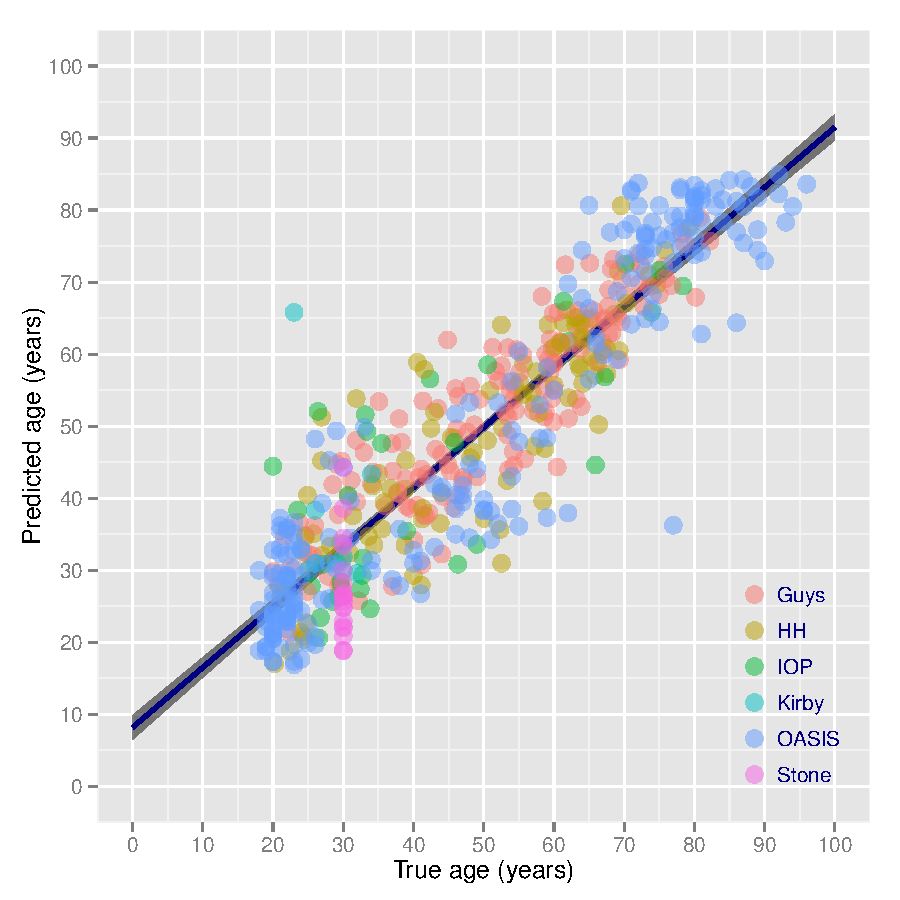
\includegraphics[width=65mm]{brainAgeBrainSegmentationPosteriors2.pdf} &
  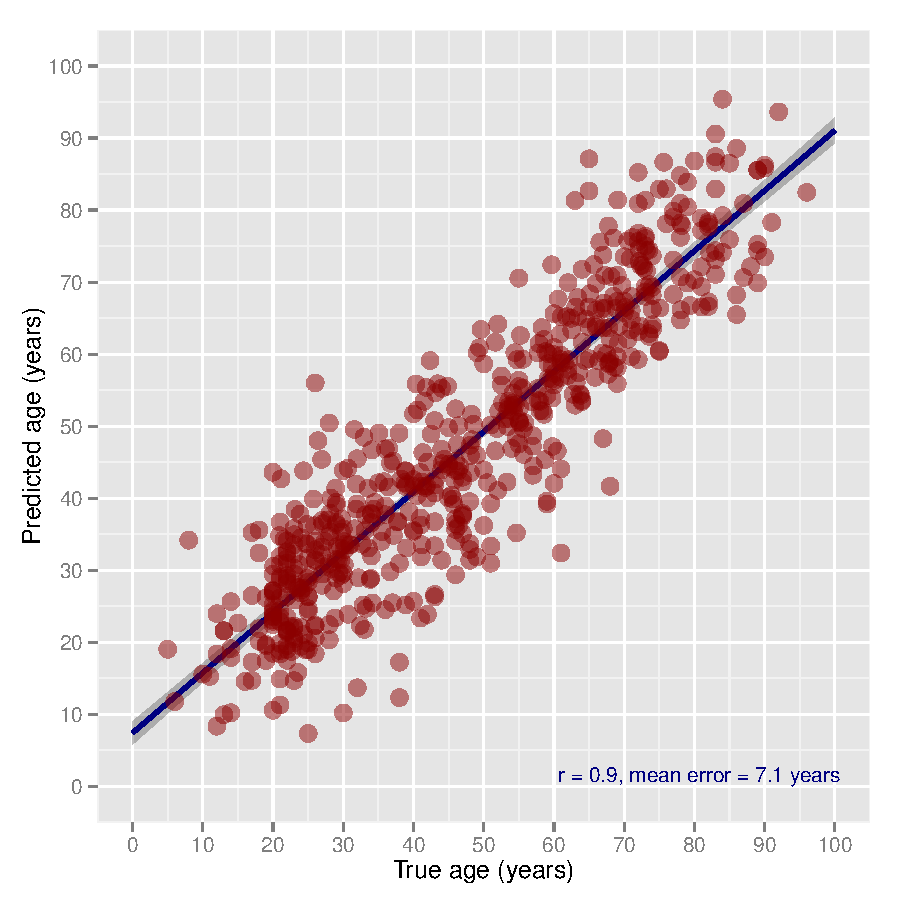
\includegraphics[width=65mm]{brainAgeCorticalThickness.pdf} \\
  (a) & (b) 
  \end{tabular}
  \caption{Results of RVM-based age prediction using (a) gray matter probability
  maps as in \cite{franke2010} and (b) cortical thickness maps both of which
  are derived from the previously described workflow.}
  \label{fig:brainAge}
\end{figure*}

In \cite{franke2010}, an estimation framework is presented for predicting 
apparent age from gray matter segmentation probability maps (denoted by the authors as {\it BrainAGE}).  
Given a normal age population spanning the age range of interest, the authors showed
how kernel regression methods can be used to reliably estimate age.  The basic processing pipeline includes 3-tissue segmentation
of a subject's T1, followed by affine registration to a common reference space (e.g.
the MNI template), smoothing (8 mm FWHM), and downsampling (8 mm 
isotropic resolution).  A principal components (PCA) model is constructed 
from the resulting aligned training image set.  The images of both the training set and 
testing set are decomposed into the bases of the PCA model which form the feature
set for relevance vector machine (RVM)-based learning and prediction, respectively. 

We applied the BrainAGE framework to the gray matter probability maps derived
from our pipeline.  We also applied the same strategy to predicting age from 
our cortical thickness images.  We randomly separated the images of each of the 
four cohorts into approximately two equal subgroups (testing and training).
Construction of the PCA model and decomposition of all images into the corresponding 
bases were performed on the training group using tools developed from the Insight Toolkit.%
\footnote{
http://www.itk.org/Doxygen/html/classitk\_1\_1ImagePCADecompositionCalculator.html  
}
We used the R-based {\it kernlab}%
\footnote{
http://rss.acs.unt.edu/Rdoc/library/kernlab/html/rvm.html
} 
package to train the RVM model and perform prediction.  Results for both
analyses  are shown in Figure \ref{fig:brainAge} (cf. Figure 3 in \cite{franke2010}).
Again, testing and training data, as well as 
R scripts used to produce the 
plots are publicly available.  
The resulting predictions for both image sets are quite similar as demonstrated 
visually in Figure 3.  The correlation coefficients and mean errors in Table 
\ref{table:brainAge} between the
two approaches are also evidence of mutual corroboration.

\subsection{Gender and Age Relationships with DiReCT Cortical Thickness}

\begin{figure}
  \centering
  \begin{tabular}{cc}
  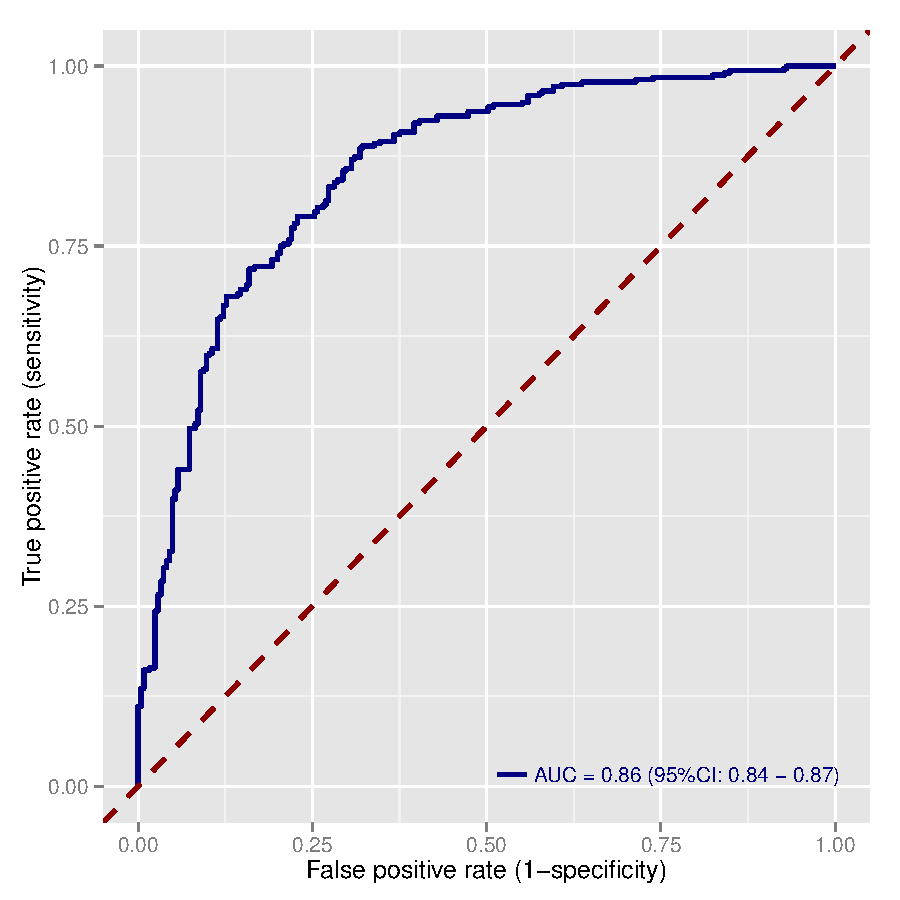
\includegraphics[width=65mm]{sexPlot.pdf} &
  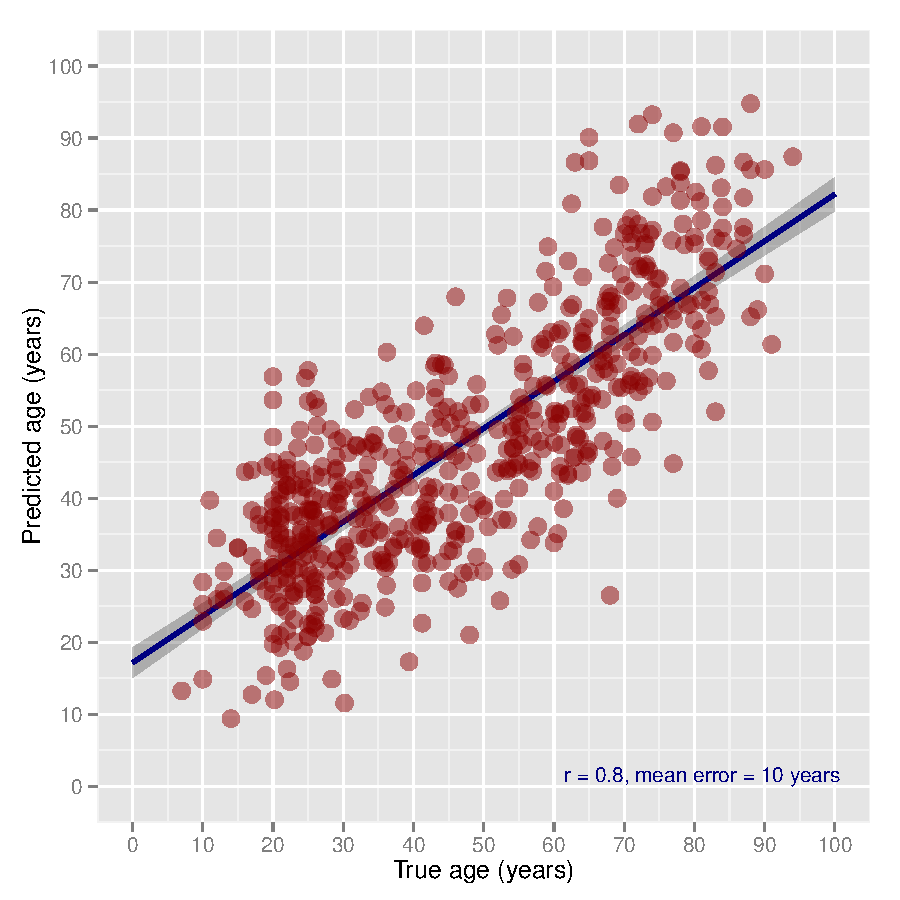
\includegraphics[width=65mm]{ageRegressionPredict.pdf} 
  \end{tabular}
  \caption{ROC curve based on a gender prediction model using total brain volume and regional thickness values.  Specifically, the model is
  }
  \label{fig:sexROC}
\end{figure}


\subsection{Gender Structural Connectivity Across Age Using Cortical Thickness}

\textcolor{red}{ Nick - should show a rendering of these networks -
  how about we residualize thickness wrt age and then look at the
  difference between male and female transitivity?  we can permute to
  get significance .... } 

\begin{figure*}
  \centering
  \begin{tabular}{c}
  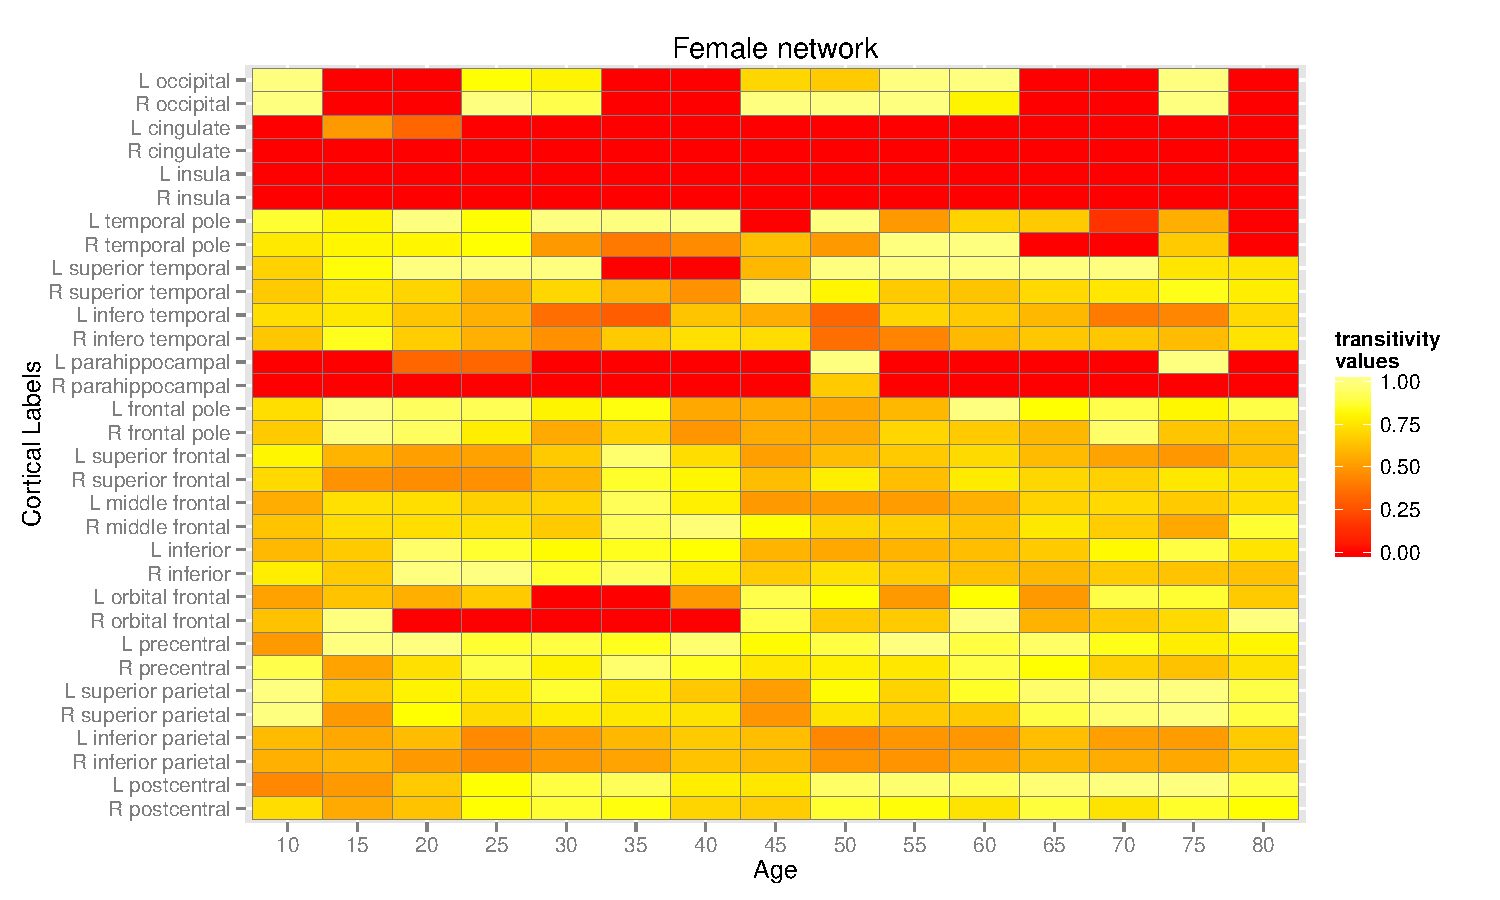
\includegraphics[width=140mm]{femaleNetwork.pdf} \\
  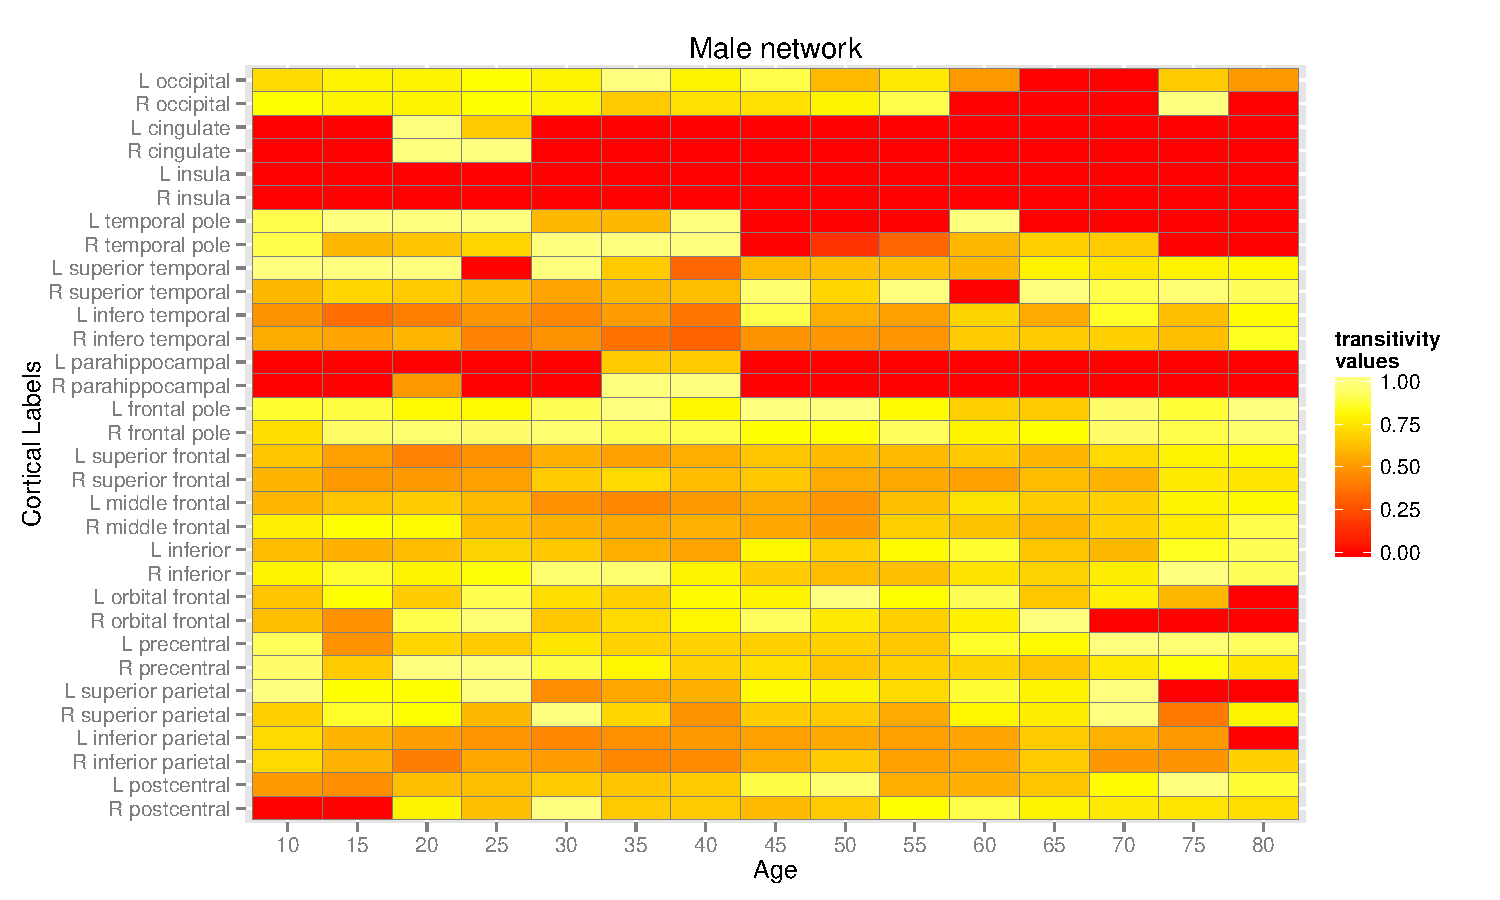
\includegraphics[width=140mm]{maleNetwork.pdf}
  \end{tabular}
  \caption{Transitivity (clustering coefficient) values across age for both the female (top)
  and male (bottom) networks.  
  }
  \label{fig:network}
\end{figure*}

As mentioned in the Introduction, cortical thickness has
been used to determine structural connectivity relationships in the brain 
where strong correlations in regional cortical 
thickness values across subjects provide evidence for anatomical
connectivity \citep{he2007,chen2008,he2008}.  Specifically, networks of neuronal
regions are thought to have small-world network properties \citep{sporns2004} 
in which clustered subnetworks are sparsely connected to other such clusters.
Measures such as the
clustering coefficient (or local transitivity) and mean shortest path length
\citep{watts1998}, are used to characterize networks in terms of their 
small-worldness.
%Although the principal purpose of this work is to showcase the 
%publicly available ANTs cortical thickness pipeline and its performance
%on open data
%(and not necessarily explore the deeper neuroscience implications of 
%the results), 
We use the compiled cortical thickness data to briefly sketch
the longitudinal variation in gender-based small-world networks of the
brain.  Note that these results are created directly from the tabulated 
cortical thickness values and processed with the R script
\verb#gender_study2.R#.

At each age between 10 and 80 years (in increments of 5), the weighted correlation
matrix for each gender is calculated from the thickness residuals 
(modeling the imaging acquisition site and total brain volume as covariates).  An undirected graph ($V \in$ \{NIREP regions\}, $E \in$ \{all NIREP pairings\})
is constructed from the correlation matrix where the graph density is specified at 25\%, i.e. only the nodal adjacencies corresponding to the top 25\% correlation values are used to create edges.    The local transitivity for a given vertex, $v_i$, with $k_i$ neighbors of the resulting graph is calculated from
\begin{align}
  transitivity(v_i) = \frac{|\{e_{jk}: v_j, v_k \in N_i, e_{jk} \in E \}|}{k_i (k_i-1)/2}.
\end{align}
Informally, this quantifies the proportion of edges between the neighbors of $v_i$ to the total number of possible edges in the neighborhood to quantify the proximity of the neighborhood to a complete graph.  Heat maps of the regional transitivity values for each
gender across age are given in Figure \ref{fig:network}.  


\subsection{Quality Control Measures}
\begin{figure}
  \centering
  \begin{tabular}{c}
  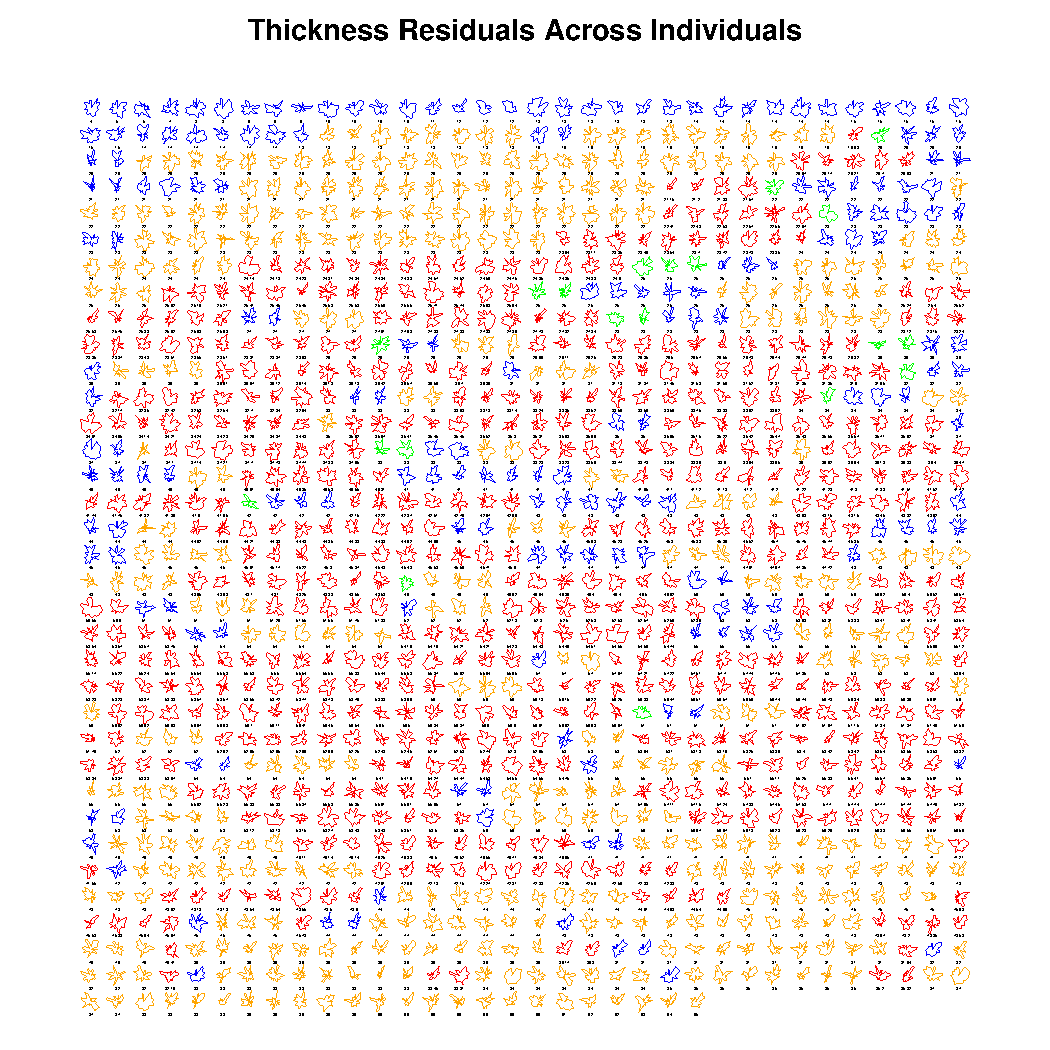
\includegraphics[width=130mm]{thicknessStarsIndividuals.pdf} 
  \end{tabular}
  \caption{Scaled thickness star plots
  }
  \label{fig:stars}
\end{figure}






